\documentclass[12pt, letterpaper]{article}
\usepackage{iarc_latex_style}
\usepackage{amssymb,amsmath,listings,url,verbatim,graphicx}

\title{Beohawk: Autonomous Quadrotor}
\begin{document}
\maketitle
\begin{people}
\name{Rustom Jehangir, Christopher Li, Yujia Zhai}
\org{University of Southern California}

\end{people}

%1) Abstract	5
\begin{abstract}
	In this paper, we introduce a Micro UAV system that can explore an unknown indoor space without the assistance of a positioning system such as GPS. The robot takes in various kind of sensing measurements, handles them with probabilistic theories, and completes tasks such as stabilization and SLAM. \todo{Finish abstract at the end} (5 points)
\end{abstract}

%2) Introduction	5
%  a) Statement of the problem 
%  b) Conceptual solution to solve the problem
%    b1) Figure of overall system architecture 
%  c) Yearly Milestones
\section{Introduction}

\subsection{Problem Statement}

For the $6^\text{th}$ International Aerial Robotics Competition (IARC 2011), an autonomous aerial vehicle under 1.5 kilograms must explore an unknown office floor, localize itself according to the environment, identify and pick up a black USB drive, and return to a handler within the given time limit. The robot may also be intelligent enough to identify mission-related features, such as signs above rooms, or observe and avoid obstacles such as surveillance devices while traversing the hallways.

\subsection{Conceptual Solution}

The Aerial Robotics Team (ART) of the USC Robotics Society (USCRS) purposes a quadrotor design of its aerial robot vehicle, \textit{Beohawk}, which consists of four motors located symmetrically at each end of an X-shape frame \todo{a figure of beohawk}. The frame of the quadrotor was custom built by our team members to be within the required weight and size range. Various sensors, the on-board computer, and other facilities are located at the center of the frame. An off-board computing station is dedicated to the majority of computational tasks; it receives data from the on-board computer, processes the data to determine future movements of the robot, and publishes operating commands back. The communication is done over a standard 802.11n network. Both computers run mission-specific programs written by our team. These programs run on the Robotic Operating System (ROS) and take advantage of many packages and tools made available by public contributors. Utilizing inertial and visual data from various sensors and processing the data with state-of-the-art algorithms, we hope to perform stabilization, navigation and mission planning on the quadrotor to complete the challenge.

\subsubsection{Figure of Overall System Architecture}

Figure \eqref{fig:architecture} shows the basic system architecture of the quadrotor. The quadrotor's low level control including stability, attitude control, altitude control, and position control are all performed by the low-level control board. This board is Arduino based and has sensor inputs and motor outputs. It also receives radio-control signals that allow control to be over-ridden by a human pilot.

\begin{figure}[h]
\centering
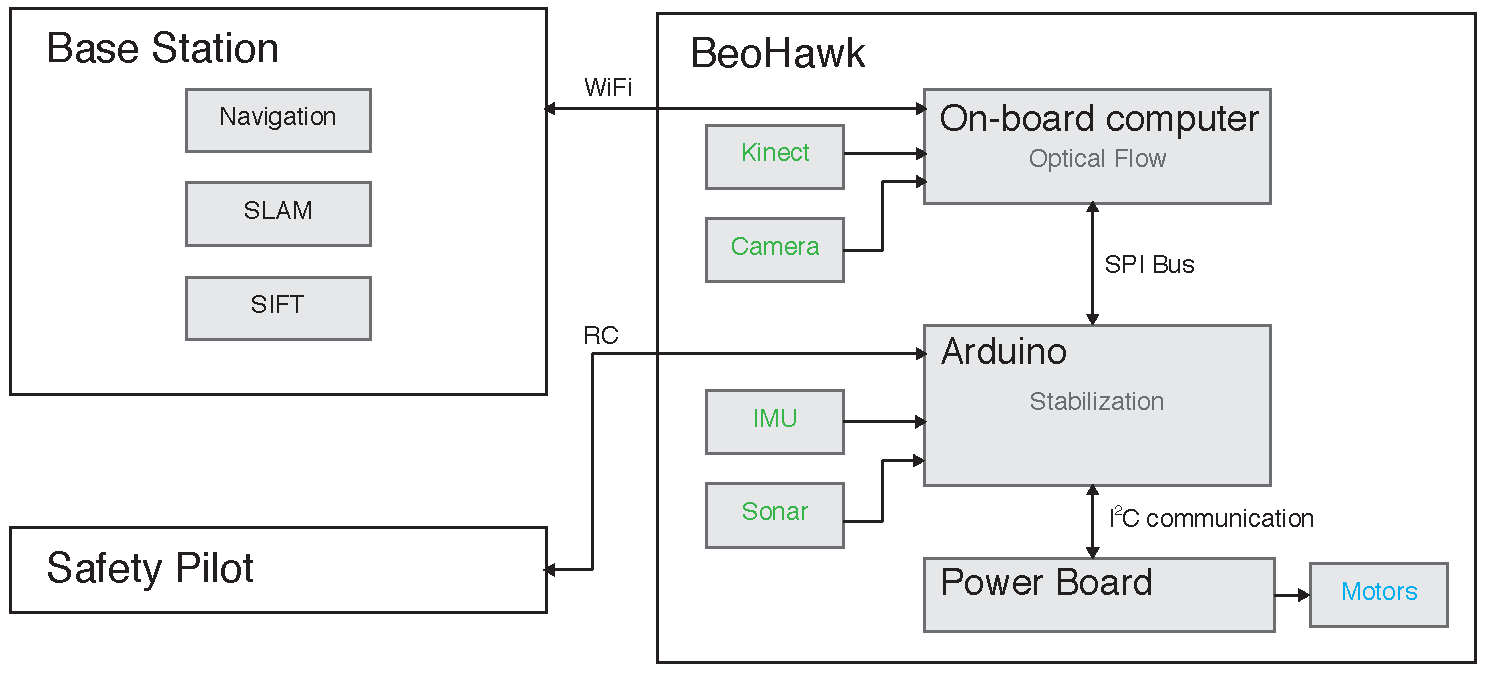
\includegraphics[width=14cm]{images/beohawk-system-arch.pdf}
\caption{General architecture of the Beohawk control system. \todo{This needs to be completed}.} 
\label{fig:architecture}
\end{figure}

\subsection{Yearly Milestones}

This is the USC Robotics Society's first appearance at IARC as well our first competition. Our hardware team has developed three models for the frame in the past two years. Our latest model uses strong, lightweight carbon fiber in the frame. The software team has researched algorithms for UAV stabilization and navigation, and has tried to develop 3D visual navigation systems through both a probabilistic approach and a graph approach, which will be discussed later in detail. Our electrical team has designed a customized circuit board to replace the commercialized alternatives (such as Arduino board). Regardless of the outcome of competition, we will continue refining hardware frames, circuit designs, software algorithms, and visualization interfaces.

% picuture of the frame (solidworks) 

%3) Air Vehicle	15
%  a) Propulsion and Lift System 
%  b) Guidance, Nav., and Control 
%    b1) Stability Augmentation System 
%    b2) Simultaneous Localization and Mapping
%    b3) Navigation
%    b4) Figure of control system architecture 
%    b5) Target Identification and Threat Avoidance
%  d) Flight Termination System
\section{Air Vehicle}

\subsection{Propulsion and Lift System}
\emph{Beohawk} has four rotors, each an equal distance from the quadrotor's center.  Two opposite motors spin clockwise and the other two spin counter-clockwise, which generates a net torque of zero.  Hence, the quadrotor does not need a separate rotor to control yaw like a conventional helicopter, and can control yaw by adjusting the proportion of rotor speeds. \todo{Todo: More details on these rotors} Quadrotors are ideal for unmanned aerial vehicles because they have simpler mechanics and require smaller rotors, which reduces the cost of the vehicle and power required to operate \cite{bib:quadrotor}.

\subsection{Guidance, Navigation, and Control}
\subsubsection{Stability Augmentation System}

Before a quadrotor flies anywhere, stabilization should be done to keep it hovering successfully in the air instead of drifting or crashing unexpectedly from its original position. Simply having equal thrust in all four motors won't solve the problem because of the asymmetrical distribution of weight across the quadrotor's body. Instead, we apply a dynamic system for measuring the drift of the quadrotor's position as well as correcting this drift.

Several sensor measurements have been proven to have strong, reliable relationships with the position (translation and/or rotation) of the robot. Monitoring their changes can give us very useful knowledge about how much the robot drifts from its original position. We use the direct-cosine matrix algorithm (DCM) to provide an optimized result of the real-time orientation of the robot \todo{Citation needed for DCM}. This algorithm utilizes the three-axis linear acceleration and angular velocity measurements from the onboard inertial measurement unit (IMU). Since linear acceleration readings from the accelerometer are more accurate in the long term while angular velocity readings from the gyroscope tend to drift through time, the DCM algorithm uses acceleration information to correct the gyroscope readings, thereby giving almost drift-free information about the robot's orientation. In addition, we also use a downward-facing camera to calculate the optical flow of salient, time-independent visual features. By doing so, we are able to figure out the motion trajectory of this camera, a technique called ``structure from motion'' \todo{[citation needed]}. A sonar sensor is also mounted on the bottom of the quadrotor. It measures a much more accurate altitude reading, and is used to improve the results of the optical flow algorithm. The combination of the DCM algorithm for the IMU and the structure-from-motion technique for the visual camera allows us to keep track of robot's linear and angular position in real time.

Finally, this system uses a PID control loop [citation needed] to handle the stabilization issue given these position-related measurements. This control loop constantly updates the proportion changes, integrals and derivatives of each monitoring variable, and to generate the motor commands that can best keep these figures away from drifting. The system also uses an Extended Kalman Filter to correct the position estimation from optical flow algorithm in order to get rid of unpredicted noises in visual feature recognition and matching.
\todo{Seems like we could use a little more on PID, I didn't proof this paragraph}

\begin{figure}[h]
\centering
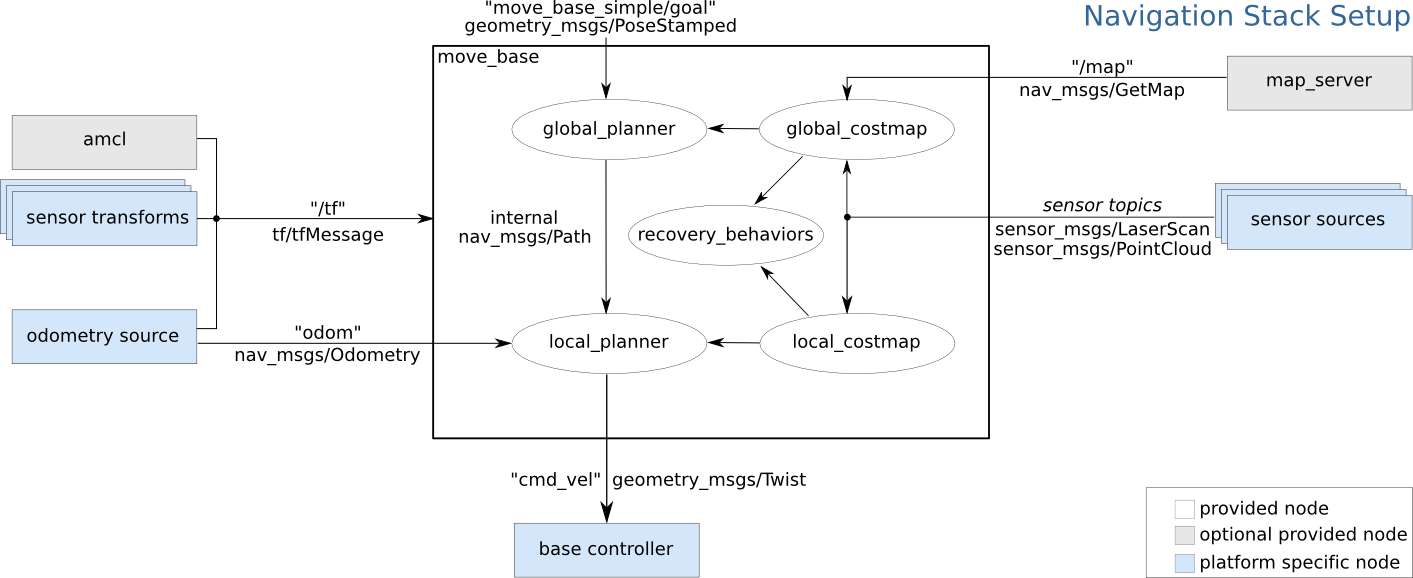
\includegraphics[width=12cm]{images/overview_tf.png}
\caption{Navigation system of Beohawk. \todo{This is a placeholder}.} 
\label{fig:navi}
\end{figure}

\subsubsection{Simultaneous Localization and Mapping}

Simultaneous localization and mapping (SLAM) has been the central problem for autonomous robots in unknown environments. The purpose of the SLAM is to predict, as accurately as possible, the position of the robot based on its knowledge of the surrounding environment.  To do this, we must obtain the 3D position of visual salient features and calculate the affine transformation of the camera through time. Combining this with the gyroscope and optical flow readings, we can set up an optimization system to reduce the effect of random errors.

In this project, we use an infrared-powered depth camera that can tell how far one given point is away from the camera. Combining this depth camera with a traditional RGB camera, we are able to create a 3D model (or ``point cloud'') of the visual perception as well as matching them in 3D to figure out the camera trajectory. Because matching every point across point clouds requires a great amount of time and energy to process, we only match the points representing the same object in the real world from different clouds. Singular value decomposition is used to process the matching result and to produce the translation and rotation matrix.

Results from the 3D visual matching and transformation calculation described above are the major source of pose estimation. To further optimize the localization result, we will use either a probabilistic system or a graph system. The probabilistic system utilizes a Monte-Carlo theory based particle filter to generate most possible result; it only depends on the probability distribution of pose at the most recent time. The graph system, on the other hand, creates a graph where vertices are the poses and edges are the transformation constraints between poses. The graph system doesn't require us to simulate the probability model of system, control, or sensing inputs, but requires more computational power to manage the graph.

\todo{a picture for particle filter and a picture for graph system}

\subsubsection{Navigation}

While we can get the 6 degree-of-freedom position and orientation status of the robot, we only need the Navigation done in 2D, because the place our robot will explore is a single plane floor. We plan to use the official 2D navigation package from ROS.

\todo{a list of states in the state machien!}

\todo{Eh, maybe not. It might turn out to be unreadable. We'll see. }

Figure \eqref{fig:navi} shows the inputs to the navigation stack. Mission control is managed with a state machine that keeps track of the current objective.  \todo{Possibly a state diagram? To finish later}

\subsubsection{Figure of Control System Architecture}

\begin{figure}[h]
\centering
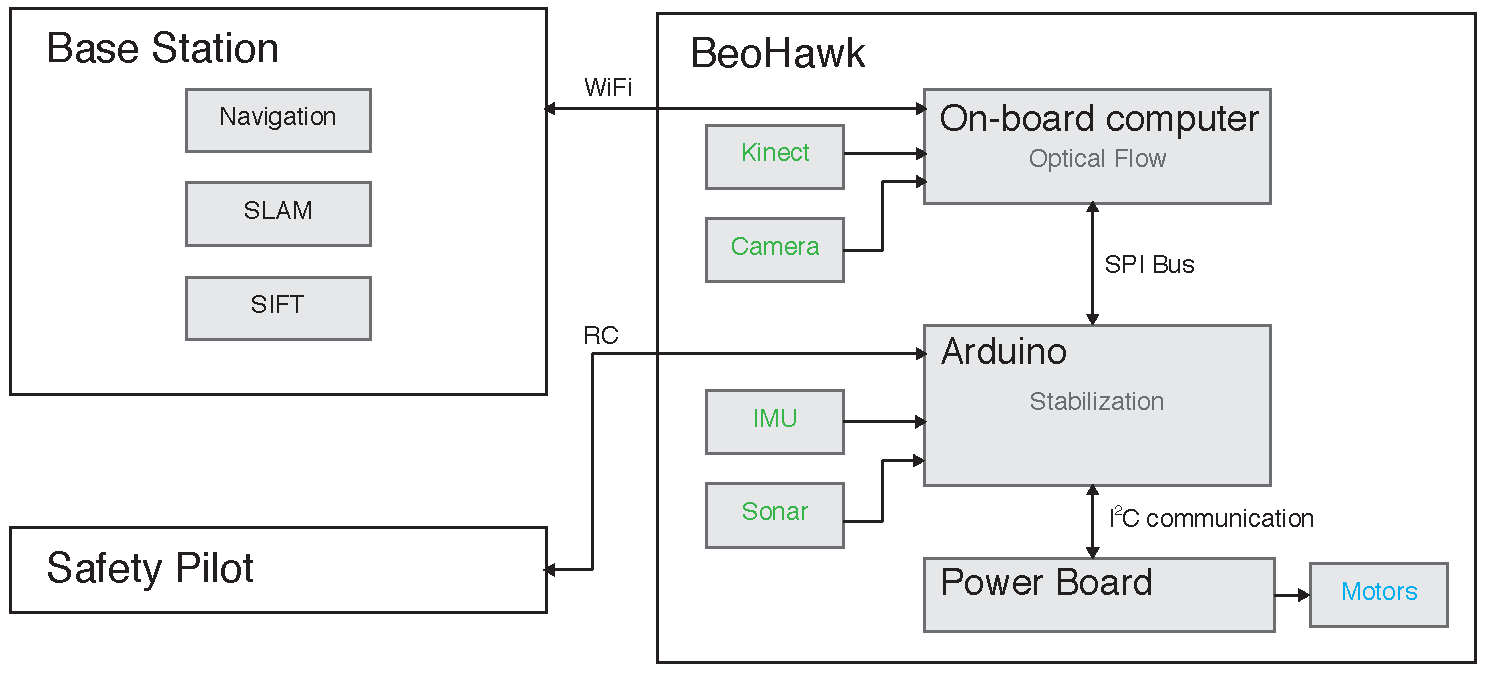
\includegraphics[width=14cm]{images/beohawk-system-arch.pdf}
\caption{Control system architecture. \todo{This needs to be completed}.} 
\label{fig:architecture}
\end{figure}

\todo{And an explanation}

\subsubsection{Target Identification and Threat Avoidance}

Since the USB is a black object located on a white table surface, an edge or contrast detection algorithm will easily identify the USB as a salient feature. While the 3D visual sensor may not be enough accurate to tell the dimension of the USB, it can sense the much larger box containing the USB and therefore helps in target identification. 

Identifying the signatures on the doors to different rooms is a tough task, because arabic characters are difficult to identify with traditional OCR technology, especially since the quadrotor may look at the signature from unknown perspective, which results in an affine transformation of the signature image that. \textit{Beohawk} uses a scale/rotation invariant feature detection algorithm called ``SURF'' to tackle this problem. The algorithm tries to match the picture it sees and the template in the database by trying numerous cases of different transformations. This algorithm has been proven successful in matching pictures regardless of scale, rotation or gradient constraints \todo{Citation needed}.

\todo{Pictures of surf in action.}

\subsection{Flight Termination System}
Because the RC controller communicates directly with the Arduino, the safety pilot can terminate the operation of the quadrotor in the event it is needed.

%4) Payload	15
%  a) Sensor Suite 
%  c) Power Management System 
%  b) Communications 

\section{Payload}
\subsection{Sensor Suite}

\subsubsection{Inertial Sensing Unit}

\todo{sensor board stuff}

\subsubsection{2D Visual Camera}

Using a downward facing camera, the quadrotor runs an optical flow algorithm on the x86 processor to reduce drift.  A second, front-facing camera captures pictures for reading the signs above the doors.  The images are published through the wireless network to the base station, which runs SIFT to detect the Chief of Security's office via the sign above the door. The front camera is also responsible for detecting the blue security light.  The bottom camera is used to identify the flash drive.

\subsubsection{3D Infrared Depth Camera}

We have installed a Microsoft Kinect on the quadrotor as a novel solution to the SLAM and navigation problem. This device serves as a depth sensing camera, which provides an image of 640x480 points at 15Hz; each point contains information at 2048 levels of sensitivity. The camera is mounted downward at a 45$^\circ$ angle from the horizon.

\subsubsection{Sonar}

Though the quadrotor has an estimate of altitude from infrared depth camera, the quadrotor also employs a downward-facing sonar to determine its altitude. A \todo{model/part number} is installed facing downwards.

\subsection{Communications}

An IEEE 802.11n network is established between an on-board computer and a ground station. This network is time-synchronized and supports functionalities on both machines to communicate with each other through the ROS message system. While camera sensors are well supported by ROS, inertial sensor data and motor command have to go through serial communication. Since serial communication has not been implemented in ROS distribution so far, we developed a serial communication node that provides a protocol for exchanging messages safely through serial communication, which greatly improves the reliability of whole system. The sensor board communicates with the power board with I$^2$C technology at \todo{n} Hz. It also connects to an RC control device that operates at \todo{n} GHz. Inertial sensors are read at \todo{n} Hz, while visual sensing streams have a rate of 30 Hz for 2D images and a rate of 15 Hz for 3D depth images.

\subsection{Power Management System}

Beohawk is powered by a 7.4V 500mAh Lithium-Polymer battery pack, which provides enough energy to run at least ten minutes. A power regulator board controls the battery and motor speed.  In the event of low power, the base station initiates a controlled descent to avoid damage to the quadrotor.

%5) Operations	10
%  a) Flight Preparations 
%    a1) Checklist(s) 
%  b) Man/Machine Interface
\section{Operations}

\subsection{Flight Preparations}
Before any flight is performed, batteries must be charged an an able human operator must be available to assume the control the RC controller.  For competition, the following checklist must be completed.

\subsubsection{Competition Checklist}
\begin{enumerate}
  \item Inspect and test hardware
  \item Launch ROS nodes
  \item Check software status
  \item Ensure RC link works
  \item Test hover in place
  \item Start mission control
\end{enumerate}

\subsection{Man-Machine Interface}
The base station displays Beohawk's current mission and status inferred from the sensor data returned by Beohawk.  If the link is terminated, Beohawk will  hover in place until the connection is restored or until the human operator assumes control. The human operator has an RC controller that communicates directly with the Arduino.


%6) Risk Reduction	15
%  a) Vehicle Status 
%    a1) Shock/Vibration Isolation 
%    a2) EMI/RFI Solutions 
%  b) Safety 
%  c) Modeling and Simulation 
%  d) Testing
\section{Risk Reduction}
\subsection{Vehicle Status}
Beohawk transmits battery information, sensor information, and current objective to the base station. 

\subsubsection{Shock/Vibration Isolation}
\todo{Keith has some stuff on this}

\subsubsection{EMI/RFI Solutions}
Because our sensors and electronics are not very sensitive to the interference from motors and wireless communications, we have not had to worry about EMI or RFI.

\subsection{Safety}

\subsection{Modeling and Simulation}
Hardware was modeled in SolidWorks.

\subsection{Testing}
We have done continuous testing on Beohawk as we developed it. \todo{hardware testing methodology}

For software, we did field tests to ensure the proper functioning of SLAM and vision algorithms.  SLAM was prototyped in MATLAB and re-written in C++ while the mission control was written in Python and has a unit test suite as well as a behavior test suite. 

\begin{table}[h]
\centering
\begin{tabular}{l  r  r  r}
                                       & Used  & Avail. & Perc. \\
  Number of Slices:                    &  684  & 4656  &  14\%  \\
  Number of Slice Flip Flops:          &  198  & 9312  &   2\%  \\
  Number of 4 input LUTs:              & 1316  & 9312  &  14\%  \\
  Number of IOs:                       &   37  &       &      \\
  Number of bonded IOBs:               &   36  &  232  &  15\%  \\
  Number of BRAMs:                     &    2  &   20  &  10\%  \\
  Number of MULT18X18SIOs:             &   10  &   20  &  50\%  \\
  Number of GCLKs:                     &    2  &   24  &   8\%  \\
\end{tabular}
\caption{Resource usage.}
\label{tab:usage}
\end{table}


%7) Conclusion	5 
\section{Conclusion (5)}
Use tables and figures to concisely state your point. A table title appears above the table it references and appears in all caps and centered, whereas a figure title appears beneath the figure and with only leading capitalization. Both table and figure titles are italicized as shown in the examples below:


%8) References	5
\bibliographystyle{IEEEbib}
\begin{thebibliography}{10}
\bibitem[1]{bib:quadrotor}
Pounds, P.; Mahony, R., Corke, P. (December 2006). ``Modelling and Control of a Quad-Rotor Robot''. In the Proceedings of the Australasian Conference on Robotics and Automation. Auckland, New Zealand.
\bibitem[1]{bib:kinectinfo} \url{http://git.marcansoft.com/?p=libfreenect.git;a=summary/}
\end{thebibliography}


\end{document}
